\section{Results: Availability, Selectivity, and Specificity}
\label{sec:results}

\subsection{Controlled decodability is robust in every cell}
\label{sec:decoding-results}

\begin{table*}[t]
\centering
\small
\setlength{\tabcolsep}{4.5pt}
\caption{Controlled decodability at the exact final visual block. Intervals are 95\% patient-cluster bootstrap intervals over 2,000 draws. The control column gives the mean AUROC over 20 recurring-type random-label maps and their 5th--95th percentile spread.}
\label{tab:decoding}
\begin{tabular}{lllccc}
\toprule
Model & Concept & Consumed module & AUROC [95\% CI] & Control mean (5--95\%) & Selectivity [95\% CI] \\
\midrule
LLaVA-1.5-7B & Effusion & model.vision\_tower.encoder.layers.22 & 0.7788 [0.7538, 0.8031] & 0.6649 (0.5750--0.7450) & 0.1139 [0.0875, 0.1404] \\
LLaVA-1.5-7B & Edema & model.vision\_tower.encoder.layers.22 & 0.8009 [0.7648, 0.8329] & 0.6649 (0.5750--0.7450) & 0.1360 [0.0994, 0.1693] \\
Qwen2.5-VL-7B & Effusion & model.visual.blocks.31 & 0.7742 [0.7488, 0.7993] & 0.6576 (0.5738--0.7476) & 0.1166 [0.0897, 0.1428] \\
\bottomrule
\end{tabular}
\end{table*}


All three final-block representations make the target label available to the fixed linear readout (Table~\ref{tab:decoding}). LLaVA Effusion reaches AUROC 0.7788 and selectivity 0.1139 (95\% CI $[0.0875,0.1404]$). LLaVA Edema reaches AUROC 0.8009 and selectivity 0.1360 ($[0.0994,0.1693]$). Qwen Effusion reaches AUROC 0.7742 and selectivity 0.1166 ($[0.0897,0.1428]$). Each selectivity interval excludes zero despite the control maps' substantial spread.

The paired decoding contrasts do not resolve a concept or architecture ordering. Within LLaVA, Edema-minus-Effusion selectivity is 0.0221 with a paired 95\% CI of $[-0.0175,0.0590]$. For Effusion, Qwen-minus-LLaVA selectivity is 0.0026 with a paired CI of $[-0.0155,0.0215]$. The cells therefore provide similarly strong availability evidence without supporting a rank claim.

\subsection{Similar availability produces different random/sham outcomes}
\label{sec:generic-results}

\begin{figure*}[t]
    \centering
    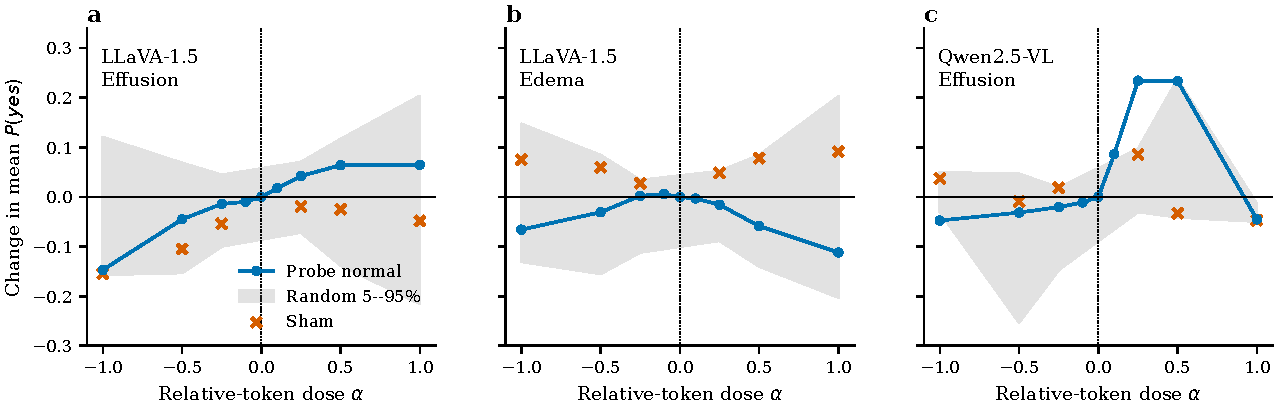
\includegraphics[width=\textwidth]{figures/fig2_dose_responses.pdf}
    \caption{\textbf{Registered dose responses at the consumed final visual block.} The blue curve is the raw change in mean $P(yes)$ under the target probe normal on the same 200 held-out images per cell. Gray bands show the 5th--95th percentile across 20 equal-norm random directions at the six controlled nonzero doses; orange crosses show the coordinate-permutation sham. The concept-consistent orientation used by the registered decision rule accounts for the negative-dose maxima in the two LLaVA cells.}
    \label{fig:dose}
\end{figure*}

Figure~\ref{fig:dose} shows the complete target dose curves and matched controls. LLaVA Effusion attains a maximum concept-consistent change of 0.1470 at $\alpha=-1$. This value exceeds the same-dose random p95 of 0.1202 but remains below the maximum absolute sham effect of 0.1546. The response is monotone over $[-0.5,0.5]$ (Spearman $\rho=1.0$), yet monotonicity does not replace the failed sham criterion.

LLaVA Edema attains 0.0659 at $\alpha=-1$. It lies inside the same-dose random interval $[-0.1304,0.1470]$ and below the maximum absolute sham effect of 0.0913. Its descriptive dose monotonicity is $\rho=-0.4286$. Edema's point estimate for controlled decoding is higher but statistically indistinguishable from Effusion's, and it does not clear the generic intervention rule.

Qwen Effusion clears the original random/sham rung. Its maximum concept-consistent change is 0.2343 at $\alpha=+0.25$, above random p95 0.0963 and the maximum absolute sham effect 0.0852. The response is nearly monotone over the registered central range ($\rho=0.9643$). This original rule establishes selectivity against generic perturbation controls. The same-dose Nodule effect of 0.2863 is descriptive at this stage and motivates the separate prospective specificity endpoint.

\begin{table*}[t]
\centering
\scriptsize
\setlength{\tabcolsep}{3.2pt}
\caption{Registered intervention outcomes. Original cohorts select the maximum concept-consistent effect over the six controlled nonzero doses; their clinical-direction endpoint was not prospectively familywise. The independent cohort locks $\alpha=+0.25$ and recomputes the maximum over five fixed clinical directions inside each of 5,000 patient-bootstrap replicates. ``Stopped at'' names the first evidentiary rung not cleared.}
\label{tab:gates}
\begin{tabular}{lllrrccccl}
\toprule
Model & Concept & Cohort & $N$ & $\alpha$ & Concept effect & Random control & $|$sham$|$ & Clinical margin [95\% CI] & Stopped at \\
\midrule
LLaVA-1.5-7B & Effusion & Original & 200 & -1.00 & 0.1470 & [-0.1566, 0.1202] & 0.1546 & --- & Random/sham \\
LLaVA-1.5-7B & Edema & Original & 200 & -1.00 & 0.0659 & [-0.1304, 0.1470] & 0.0913 & --- & Random/sham \\
Qwen2.5-VL-7B & Effusion & Original & 200 & +0.25 & 0.2343 & [-0.0299, 0.0963] & 0.0852 & --- & Clinical directions \\
Qwen2.5-VL-7B & Effusion & Independent & 400 & +0.25 & 0.1945 & p95=0.0878 & 0.0157 & -0.0573 [-0.0694, -0.0450] & Clinical directions \\
\bottomrule
\end{tabular}
\end{table*}


\subsection{Independent rows separate generic selectivity from clinical specificity}
\label{sec:specificity-results}

\begin{figure*}[t]
    \centering
    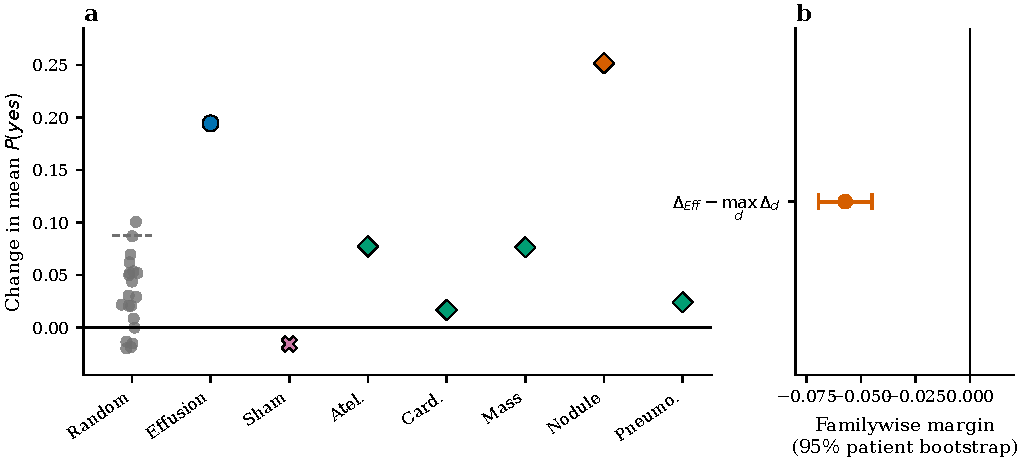
\includegraphics[width=0.82\textwidth]{figures/fig3_direction_specificity.pdf}
    \caption{\textbf{Qwen Effusion replicates above generic controls but not fixed clinical directions.} \textbf{(a)} Changes in mean $P(yes)$ at $\alpha=+0.25$ on 400 patients absent from the original cohort. The random group contains 20 directions; its dashed segment marks p95. Diamonds show the five fixed unrelated clinical normals. \textbf{(b)} The Effusion-minus-maximum-unrelated statistic with its two-sided 95\% patient-bootstrap interval; the registered one-sided 95\% lower bound is $-0.0678$. Nodule realizes the point-estimate maximum.}
    \label{fig:specificity}
\end{figure*}

The independent cohort reproduces Qwen's generic response (Figure~\ref{fig:specificity}). Effusion changes mean $P(yes)$ by 0.1945, above random p95 0.0878 and absolute sham 0.0157. This result uses 400 distinct patients, all absent from the original intervention cohort, and retains the discovery-locked dose.

The clinical comparison reverses the interpretation of that generic pass. Nodule changes mean $P(yes)$ by 0.2519 and realizes the maximum unrelated-direction effect. The reported Effusion-minus-maximum-unrelated margin is $-0.0573$. When the maximum over all five fixed clinical directions is recomputed in each bootstrap replicate, its two-sided 95\% CI is $[-0.0694,-0.0450]$ and its one-sided 95\% lower bound is $-0.0678$. The direction-specific conjunction therefore fails despite replicated random/sham selectivity.

\subsection{The three-rung finding chain}

The results form one ordered finding. First, every target is robustly available to the same-capacity linear readout. Second, the two LLaVA probe normals stop at the random/sham rung, showing that availability does not determine generic intervention selectivity. Third, Qwen Effusion passes generic controls twice but stops at the clinical-direction rung, showing that generic selectivity does not determine clinical specificity. The location, dose, controls, and uncertainty calculation identify the rung at which each interpretation is supported.
